% !TEX root = ../team-report.tex
% ERA-Großpraktikum: Team Bericht -- Gruppendynamik

\section{Gruppendynamik und Kommunikation}
\label{team:group}

Die wohl wichtigste Säule bei gemeinsamer Arbeit in einem Team, ob für die
Entwicklung eines Assembler-Simulators oder jedes sonstige Bestreben, ist die
Kommunikation innerhalb der Gruppe. Insbesondere wird diese Säule essentiell,
wenn sich das Team nicht jeden Tag im Büro begegnet, sondern verstreut und
verteilt, womöglich sogar in verschiedenen Teilen der Welt, am gemeinsamen Ziel
arbeitet. Da die meisten Mitglieder des \erasim{}-Teams aufgrund des
Studentenlebens, wie bereits besprochen, nur unregelmäßig verfügbar waren, und
der Gruppenleiter auch den Großteil des Entwicklungszeitraums in London Praktika
absolvierte, war auch für \erasim{} die Instandhaltung effektiver
Kommunikationskanäle und regelmäßiger, virtueller oder persönlicher, Treffen von
höchster Wichtigkeit. Die folgenden Abschnitte wollen einen Einblick geben, auf
welche Weise uns diese Instandhaltung via \emph{Slack}, \emph{Hangouts} und
persönlichen Treffen gelungen ist. Hierbei wollen wir auch die empfundene
Dynamik im Team erörtern.

% !TEX root = ../team-report.tex
% ERA-Großpraktikum: Team Bericht -- Gruppendynamik (Slack)

\subsection{Slack}
\label{team:group-slack}

Unser wichtigster Kommunikationskanal war die Teamchat-Software \emph{Slack}.
Slack erlaubt sowohl persönliche, "vier-Augen" Chats, als auch die Aufspaltung
der Diskussion in themenspezifische \emph{Kanäle} (engl. \emph{Channels}). Bei
der Entwicklung von \erasim{} verteilten wir unsere Kommunikation hierbei auf
zwei Arten von Kanälen: \emph{Teamkanäle} und \emph{Topic-Kanäle}.

Teamkanäle waren jene Kanäle, in denen jede Untergruppe von \erasim{}, also
\emph{Arch, Core, Parser} und \emph{GUI}, Diskussionen führen konnten, die sich
rein mit den Aspekten der Entwicklung von \erasim{} befassten, die jeder Gruppe
entsprachen. In diesen Chats wurde über den Fortschritt sowie aufgetretene
Probleme eines einzelnen Mitglieds der Untergruppe berichtet, wichtige
Informationen zur Entwicklungsumgebung diskutiert (z.B. eine neue Qt Version
oder die Veröffentlichung einer neuen RISC-V Spezifikation) oder auf scheiternde
Tests aufmerksam gemacht. Wichtig hierbei war insbesondere, dass diese Teamchats
nicht für die Untergruppe privat, sondern für das ganze \erasim{} Team
öffentlich war. Somit konnten auch von Mitgliedern anderer Untergruppen Fragen
gestellt bzw. wichtige Entwicklungen mitgeteilt werden. Wollte beispielsweise
ein Mitglied des Core wissen, auf welchem Wege man am besten die Registergröße der
momentan geladenen Architektur abruft, so konnte er oder sie diese Frage im
Arch-Chat stellen und ihm oder ihr wurde meist auch schnell geholfen.

Neben Teamkanälen wurde auch kräftig in den Topickanälen diskutiert. Ein
Topickanal beschränkte sich auf ein spezifisches Gebiet der Entwicklung oder
anderen Themen. Ein wichtiger und vielgenutzter Kanal war beispielsweise der
C\texttt{++} Channel. In diesem konnten Fragen zu C++ gestellt, stilistische
Aspekte des Google Style Guides diskutiert oder auch bezüglich kryptischen
Kompilierfehlern nachgefragt werden. Mitglieder mit mehr C++ Erfahrung konnten
diese Fragen dann beantworten oder auf entsprechende Ressourcen hinweisen. Ein
anderer Topickanal war \emph{report} genannt, in welchem die Planung und
Fertigstellung des ersten und finalen Berichts besprochen wurde. Ein weiteres
nützliches Feature von Slack ist die Integration mit externen Dienstleistungen.
So gab es einen weiteren Topickanal, genannt \emph{notifications}, in welchen
wir unseren Test-Server \emph{Travis} integriert hatten. Immer wenn unsere Tests
auf Travis scheiterten oder erfolgreich waren, erhielten wir in diesem Kanal
eine Benachrichtigung. Dadurch musste man auch nicht mehr die Website von Travis
besuchen, um den Status der Tests zu erfahren.

In Summe waren gegen Ende der Entwicklung auf Slack 12 Kanäle offen --- 4
Teamkanäle und 8 Topickanäle. In diesen Kanälen und über private Chats wurden
über den gesamten Entwicklungszeitraum hinweg gesammelt 14,800 Nachrichten
ausgetauscht. \autoref{fig:slack} schlüsselt diese Zahl weiter auf.

\begin{figure}[h!]
  \centering
  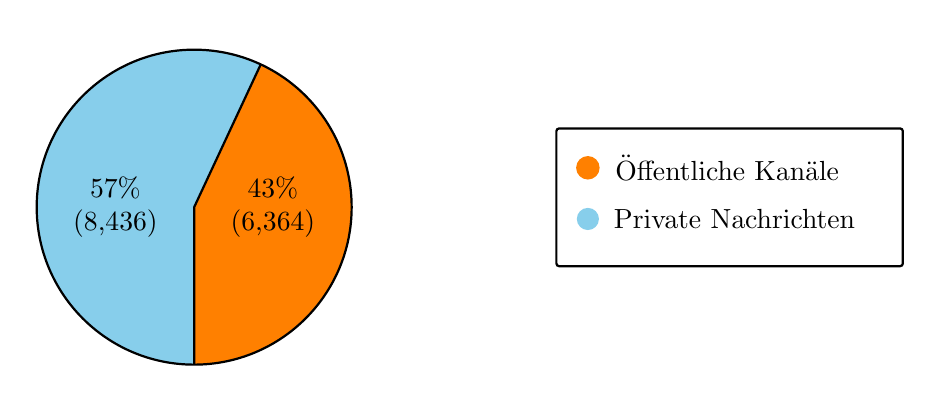
\begin{tikzpicture}[thick]

    % Public Channels
    \fill [SkyBlue]
          (0, -2) -- (0, 0) -- (65:2cm)
          arc [radius=2cm, start angle=65, end angle=270];

    % Direct Messages
    \fill [orange]
          (0, -2) -- (0, 0) -- (65:2cm)
          arc [radius=2cm, start angle=65, end angle=-90];

    % Pie border
    \draw (0, 0) circle [radius=2cm];

    % Sector border
    \draw (0, -2) -- (0, 0) -- (65:2cm);

    % Labels
    \node at (-1, 0) [align=center] {57\% \\ (8,436)};
    \node at (+1, 0) [align=center] {43\% \\ (6,364)};

    % Legend
    \path (5, 0.5) coordinate [fill, orange, circle, inner sep=3pt] (public)
          node [right] {\hspace{0.1cm} Öffentliche Kanäle};
    \fill [SkyBlue] (public)+(0, -0.65cm) circle [radius=4pt]
          node [right] {\hspace{0.2cm}\color{black} Private Nachrichten};
    \draw [thick, rounded corners=1pt]
          (public)+(-0.4, +0.5) rectangle ++(4, -1.25);

  \end{tikzpicture}
  \caption{Eine Aufschlüsselung der über Slack versendeten
  Nachrichten. Der relative Anteil und die absolute Anzahl an Nachrichten in
  öffentlichen Kanälen sind in Orange eingezeichnet, private Nachrichten in
  Türkis. Insgesamt wurden über 10 Monate hinweg 14,800 Nachrichten verschickt.}
  \label{fig:slack}
\end{figure}

\vspace{-0.5cm}

% !TEX root = ../team-report.tex
% ERA-Großpraktikum: Team Bericht -- Gruppendynamik (Hangouts)

\subsection{Hangouts}
\label{team:group-slack}

Mag die Kommunikation über Slack in unserem Team auch schon sehr effektiv
gewesen sein, so ist natürlich dennoch ein gewisser Grad an persönlichem,
verbalem Austausch für ein gutes Klima im Team unerlässlich. Besonders Brainstorming, das Besprechen von Designs für
Softwarekomponenten oder weitere Diskussionen ließen sich besser mündlich statt schriftlich erledigen. In unserem Team konkretisierte sich die verbale Kommunikation
insbesondere virtuell, über \emph{Hangouts}\footnote{\emph{Google Hangouts}
(\url{http://hangouts.google.com}) ist ein VoIP-Service von Google, Inc.}. Es
traf sich meist mehrmals im Monat jede Untergruppe per Hangout,

\vspace{0.2cm}
\pagebreak

um den nächsten Sprint bzw. die nächsten Schritte zu planen. Bei diesen Hangouts
stand es auch Mitgliedern anderer Gruppen frei, teilzunehmen, um beispielsweise
über die Integration zweier Module zu diskutieren. Teilweise nahm auch der
Gesamtgruppenleiter an den Hangouts anderer Gruppen bei, um die Entwicklung zu
überprüfen und womöglich technische Ratschläge zu geben. Letztlich gab es zu
seltenen (aber wichtigen) Anlässen auch Hangouts, bei denen alle Mitglieder
präsent waren. Diese waren aufgrund der Größe der Gruppe jedoch organisatorisch
schwer zu planen und zu koordinieren.

% !TEX root = ../team-report.tex
% ERA-Großpraktikum: Team Bericht -- Gruppendynamik (Hangouts)


\subsection{Persönliche Treffen}
\label{team:group-pers}

Neben Diskussionen auf Slack oder Hangouts gab es auch einige Male persönliche
Treffen, bei denen sich die ganze Gruppe und manchmal auch die
Projektbetreuung persönlich trafen. Diese Treffen fanden ganz am Anfang des
Großpraktikums, im April und Mai, häufiger, im späteren Teil des
Entwicklungszeitraums weniger häufig statt. Es gibt zwei hauptsächliche Gründe,
wieso wir die Kommunikation über Slack und Hangouts bevorzugten. Zum einen ist
die Planung eines Treffens von 10 bis 12 Personen platz- und zeittechnisch eine
große Herausforderung. Zum anderen ergab sich schlussendlich aus der physischen
Präsenz der Mitglieder auch kein nennenswerter Vorteil gegenüber einem viel
praktikableren virtuellen Treffen via Hangouts.

% !TEX root = ../team-report.tex
% ERA-Großpraktikum: Team Bericht -- Gruppendynamik (Hangouts)

\subsection{Analyse und Diskussion}
\label{team:group-anal}

Im Rückblick war die Kommunikation auf Slack zweifellos der wichtigste Baustein
der Entwicklung von \erasim{}, da dieser erst sämtliche weitere Aspekte,
insbesondere die technischen, ermöglichte. Würde man die Gruppendynamik
bezüglich der Kommunikation auf Slack evaluieren, so könnte man sagen, dass die
aktive, regelmäßige Beteiligung an Diskussionen aller Mitglieder ein höchst
erfreuliches Merkmal unseres Entwicklungsalltags war. Unter den Mitgliedern, die
bis zum Schluss im \erasim{} Team waren (also nicht ausgetreten sind), gab
es niemanden, der nicht mehr oder minder täglich an Diskussionen teilnahm,
Fragen beantwortete, Fragen stellte und sein oder ihr Wissen mit anderen teilte.

Die Tatsache, dass die Kommunikation auf Slack nur schriftlich und nicht verbal
vonstatten ging, hat unsere Effektivität nicht beschränkt. Vielmehr finden wir,
dass Slack gegenüber verbaler Kommunikation den Vorteil aufweist, dass sich auch
schüchternere Mitglieder eher zu Wort trauten. Auch war der Nachteil verbaler
Kommunikation in einer Gruppe, dass nur eine Person zu einem Zeitpunkt sprechen
sollte und die Auswahl dieser Person bekanntlich oftmals chaotisch und
ineffizient ist, bei Chats nicht gegeben. Nichtsdestotrotz sind wir uns auch
einig, dass die Entscheidung, wichtigere oder komplexere Diskussionen auf
Hangouts auszulagern, sowie auch sporadisch persönliche Treffen zu veranstalten,
richtig war. Summa summarum würden wir unsere "Kommunikationshierarchie", also
$\text{Slack} \succ \text{Hangouts} \succ \text{Treffen}$, als äußerst effektiv
beurteilen.

